% =============================================================================
% Presentation: Tian (2024, REStat)
% International Trade Liberalization and Domestic Institutional Reform
% =============================================================================
\documentclass[10pt,aspectratio=169,t]{beamer}

% --- Theme & Colors ---
\usetheme{Madrid}
\usecolortheme{whale}
\useinnertheme{rectangles}
\setbeamertemplate{navigation symbols}{}
\setbeamertemplate{footline}{%
  \leavevmode%
  \hbox{%
    \begin{beamercolorbox}[wd=.35\paperwidth,ht=2.5ex,dp=1.125ex,leftskip=.3cm]{author in head/foot}%
      \usebeamerfont{author in head/foot}\insertshortauthor
    \end{beamercolorbox}%
    \begin{beamercolorbox}[wd=.40\paperwidth,ht=2.5ex,dp=1.125ex,center]{title in head/foot}%
      \usebeamerfont{title in head/foot}\insertshorttitle
    \end{beamercolorbox}%
    \begin{beamercolorbox}[wd=.25\paperwidth,ht=2.5ex,dp=1.125ex,rightskip=.3cm plus1fil]{date in head/foot}%
      \usebeamerfont{date in head/foot}\insertshortdate{}\hfill\insertframenumber/\inserttotalframenumber
    \end{beamercolorbox}}%
  \vskip0pt%
}
\setbeamerfont{frametitle}{series=\bfseries}
\setbeamertemplate{itemize items}[triangle]

% --- Packages ---
\usepackage{fontspec}
\setmainfont{Times New Roman}
\setsansfont{Times New Roman}
\usepackage{amsmath,amssymb}
\usepackage{booktabs}
\usepackage{graphicx}
\usepackage{tikz}
\usetikzlibrary{arrows.meta,positioning,calc,decorations.pathreplacing,shapes.geometric}
\usepackage{adjustbox}
\usepackage{multirow}
\usepackage{array}
\usepackage{xcolor}
\usepackage{hyperref}
\usepackage{appendixnumberbeamer}

% --- Custom Colors ---
\definecolor{darkblue}{RGB}{0,51,102}
\definecolor{alertred}{RGB}{178,34,34}
\definecolor{resultgreen}{RGB}{0,100,0}
\definecolor{lightgray}{RGB}{245,245,245}
\definecolor{mechblue}{RGB}{70,130,180}

% --- Custom Commands ---
\newcommand{\hlight}[1]{\textcolor{darkblue}{\textbf{#1}}}
\newcommand{\rmark}[1]{\textcolor{alertred}{#1}}
\newcommand{\gmark}[1]{\textcolor{resultgreen}{#1}}
\newcommand{\asinh}{\operatorname{sinh}^{-1}}

% --- Title Information ---
\title[Tian (2024, REStat)]{International Trade Liberalization and\\Domestic Institutional Reform}
\subtitle{Effects of WTO Accession on Chinese Internal Migration Policy}
\author[Yuan Tian]{Yuan Tian\\{\small University of Nottingham}}
\date{\textit{The Review of Economics and Statistics}, May 2024, 106(3): 794--813}
\institute[Presented by Christopher]{Presented by Christopher}

% =============================================================================
\begin{document}

% --- TITLE SLIDE ---
\begin{frame}[plain]
\titlepage
\end{frame}

% --- OUTLINE ---
\begin{frame}{Outline}
\tableofcontents
\end{frame}

% =============================================================================
\section{Motivation and Research Question}
% =============================================================================

\begin{frame}{Why Does This Paper Matter?}
\begin{columns}[T]
\begin{column}{0.55\textwidth}
\textbf{Central Thesis:}
\medskip

Trade liberalization increases the \hlight{effective cost} of maintaining economic institutions that impede factor reallocation.

\bigskip
\textbf{The Setting:}
\begin{itemize}
    \item China's WTO accession (Nov.\ 2001) $\rightarrow$ large reduction in tariffs on Chinese exports
    \item China's Hukou system: a legacy institution regulating internal migration
    \item Around 2001: central gov't allowed prefectures to reform Hukou locally
\end{itemize}

\bigskip
\textbf{Research Question:}\\[4pt]
\rmark{Did export-market liberalization cause Chinese local governments to relax migration restrictions?}
\end{column}
\begin{column}{0.42\textwidth}
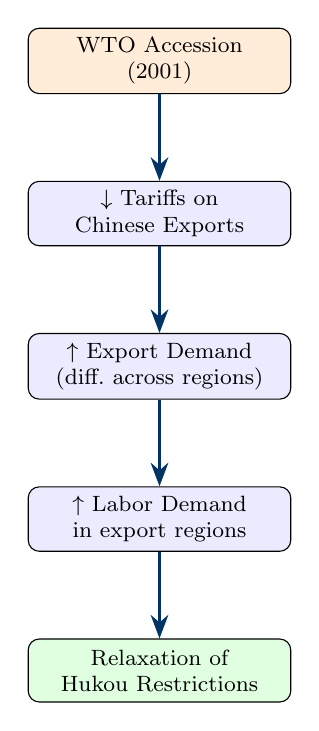
\begin{tikzpicture}[
    node distance=1.1cm,
    every node/.style={font=\footnotesize},
    box/.style={draw, rounded corners, fill=blue!8, text width=3.1cm, align=center, minimum height=0.8cm},
    arrow/.style={-{Stealth[length=3mm]}, thick, darkblue}
    ]
    \node[box, fill=orange!15] (wto) {WTO Accession\\(2001)};
    \node[box, below=of wto] (tariff) {$\downarrow$ Tariffs on\\Chinese Exports};
    \node[box, below=of tariff] (export) {$\uparrow$ Export Demand\\(diff.\ across regions)};
    \node[box, below=of export] (labor) {$\uparrow$ Labor Demand\\in export regions};
    \node[box, below=of labor, fill=green!12] (hukou) {Relaxation of\\Hukou Restrictions};
    \draw[arrow] (wto) -- (tariff);
    \draw[arrow] (tariff) -- (export);
    \draw[arrow] (export) -- (labor);
    \draw[arrow] (labor) -- (hukou);
\end{tikzpicture}
\end{column}
\end{columns}
\end{frame}

% --- Contribution ---
\begin{frame}{Contributions to the Literature}
\begin{enumerate}
    \item \hlight{Trade $\rightarrow$ Institutions:} Direct empirical evidence that trade liberalization causes changes in observed regulations
    \begin{itemize}
        \item Complements Acemoglu et al.\ (2005), Trefler \& Puga (2014), Khandelwal et al.\ (2013)
        \item Unlike inferring institutional change from trade patterns, this paper \rmark{directly measures} regulatory changes using text data
    \end{itemize}
    
    \medskip
    \item \hlight{Novel Dataset:} First prefecture-level panel of migration regulations (1978--2016)
    \begin{itemize}
        \item 4,273 migrant-related regulations, hand-coded + NLP validation (RF, MLP, CNN)
    \end{itemize}
    
    \medskip
    \item \hlight{Labor Mobility as Endogenous:} Labor market frictions respond to economic incentives
    \begin{itemize}
        \item Extends Tombe \& Zhu (2019), Fan (2019), Ma \& Tang (2020) who take frictions as given
    \end{itemize}
    
    \medskip
    \item \hlight{Fiscal Competition:} Prefectures compete to attract migrants by providing amenities
    \begin{itemize}
        \item Related to Tiebout (1956), Fajgelbaum et al.\ (2019)
    \end{itemize}
\end{enumerate}
\end{frame}

% =============================================================================
\section{Institutional Background: The Hukou System}
% =============================================================================

\begin{frame}{The Hukou System: China's Internal Migration Barrier}
\begin{columns}[T]
\begin{column}{0.52\textwidth}
\textbf{What is Hukou?}
\begin{itemize}
    \item Internal registration system: each person tied to a \hlight{location} and \hlight{sector} (agricultural vs.\ non-agricultural)
    \item Living outside Hukou prefecture requires \textit{temporary registration}
    \item Even legal migrants face diminished access to:
    \begin{itemize}
        \item Medical insurance
        \item Public schools for children
        \item Formal employment
    \end{itemize}
\end{itemize}

\bigskip
\textbf{Scale:}
\begin{itemize}
    \item 2000: 11\% of population lived outside Hukou prefecture
    \item 2010: 260 million migrants ($\approx$ 2$\times$ the 2000 figure)
    \item In 2016: 22.5\% of world population subject to similar systems
\end{itemize}
\end{column}
\begin{column}{0.45\textwidth}
\textbf{Timeline of Reform:}
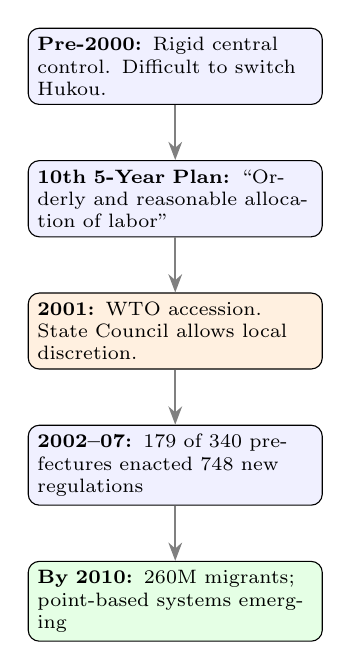
\begin{tikzpicture}[
    node distance=0.7cm,
    every node/.style={font=\scriptsize},
    event/.style={draw, rounded corners, fill=blue!6, text width=3.5cm, align=left, minimum height=0.6cm}
    ]
    \node[event] (a) {\textbf{Pre-2000:} Rigid central control. Difficult to switch Hukou.};
    \node[event, below=of a] (b) {\textbf{10th 5-Year Plan:} ``Orderly and reasonable allocation of labor''};
    \node[event, below=of b, fill=orange!12] (c) {\textbf{2001:} WTO accession. State Council allows local discretion.};
    \node[event, below=of c] (d) {\textbf{2002--07:} 179 of 340 prefectures enacted 748 new regulations};
    \node[event, below=of d, fill=green!10] (e) {\textbf{By 2010:} 260M migrants; point-based systems emerging};
    
    \draw[-{Stealth}, thick, gray] (a.south) -- (b.north);
    \draw[-{Stealth}, thick, gray] (b.south) -- (c.north);
    \draw[-{Stealth}, thick, gray] (c.south) -- (d.north);
    \draw[-{Stealth}, thick, gray] (d.south) -- (e.north);
\end{tikzpicture}
\end{column}
\end{columns}
\end{frame}

% =============================================================================
\section{Data: Measuring Migration Regulations}
% =============================================================================

\begin{frame}{Data Collection: A Novel Dataset on Hukou Policies}
\textbf{Source:} \texttt{pkulaw.com} --- most comprehensive database on Chinese government regulations\\[4pt]
Covers 332 of 340 prefectures; keyword search on: \textit{non-Hukou population, migrant worker, temporary residence, Hukou}

\bigskip
\begin{columns}[T]
\begin{column}{0.48\textwidth}
\textbf{Step 1: Identify} migrant-related regulations\\
$\rightarrow$ 4,273 regulations (1978--2016)\\[2pt]
\quad 2,915 prefecture-level; 1,358 province-level

\bigskip
\textbf{Step 2: Classify} by topic:
\begin{enumerate}\setlength{\itemsep}{1pt}
    \item Work-related (wages, contracts, training)
    \item Social insurance (medical, pension, injury)
    \item Local public goods (schools, vaccination)
    \item Hukou admin (fees, procedures)
    \item Family planning
    \item Miscellaneous
\end{enumerate}
\end{column}
\begin{column}{0.48\textwidth}
\textbf{Step 3: Score} migrant-friendliness on $\{-2, -1, 0, 1, 2\}$:
\begin{itemize}\setlength{\itemsep}{2pt}
    \item[+2] Complete, executable guideline on specific issue (e.g., mandatory wage deposits)
    \item[+1] Enforcement of existing rules (e.g., timely payment before Chinese New Year)
    \item[0] Purely administrative/logistic
    \item[$-1$] Enforcement restricting access
    \item[$-2$] Guideline depriving migrant rights
\end{itemize}

\bigskip
\textbf{Step 4: Cumulate} scores to year $t$:
$$\text{Score}_{i,t} = \sum_{s=1978}^{t} \text{score}_{i,s}$$
\end{column}
\end{columns}
\end{frame}

% --- NLP Validation ---
\begin{frame}{Validation: Machine Learning Coding}
\textbf{Concern:} Subjectivity of manual coding\\[4pt]
\textbf{Solution:} Triple-coding (author + 2 RAs) + 3 NLP methods on 686 training regulations

\bigskip
\begin{columns}[T]
\begin{column}{0.55\textwidth}
\begin{table}[h]
\centering\footnotesize
\begin{tabular}{@{}lccc@{}}
\toprule
& \textbf{Random} & \textbf{MLP} & \textbf{CNN w/} \\
& \textbf{Forest} & & \textbf{Embedding} \\
\midrule
Method type & Decision tree & Neural net & Neural net \\
Text features & Words + freq. & Words + freq. & Words + context \\
Training accuracy & 684/686 & 652/686 & 624/686 \\
Corr.\ w/ manual & 0.734 & 0.728 & 0.712 \\
\bottomrule
\end{tabular}
\end{table}

\medskip
All NLP codings produce \hlight{very similar} empirical results $\rightarrow$ robust to coding methodology

\end{column}
\begin{column}{0.42\textwidth}
\textbf{Key Words from RF Classification:}\\[4pt]
Top importance: \textit{floating population}, \textit{migrant worker}, \textit{temporary residence permit}

\medskip
Positive sentiment words: \textit{timeliness}, \textit{effectiveness}, \textit{normativity}

\medskip
Negative sentiment words: \textit{rental housing}, \textit{public security}

\bigskip
\textbf{Prefecture-level correlation} between manual and RF scores (2001--07 change): \rmark{$\rho = 0.96$}
\end{column}
\end{columns}
\end{frame}

% --- Descriptive Patterns ---
\begin{frame}{Descriptive Evidence: A Structural Break After 2001}
\begin{columns}[T]
\begin{column}{0.48\textwidth}
\textbf{Figure 2(a): Regulation Trends}

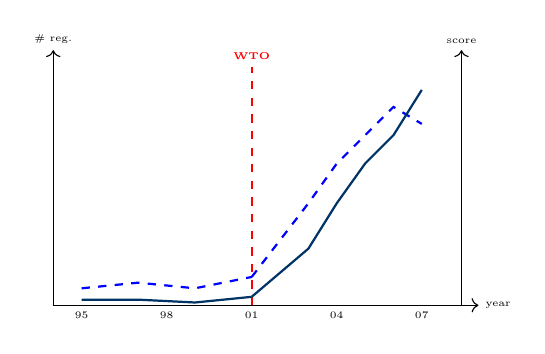
\begin{tikzpicture}[scale=0.72, transform shape]
\begin{scope}
    % Axes
    \draw[->] (0,0) -- (7.5,0) node[right] {\tiny year};
    \draw[->] (0,0) -- (0,4.5) node[above] {\tiny \# reg.};
    \draw[->] (7.2,0) -- (7.2,4.5) node[above] {\tiny score};
    
    % Year labels
    \foreach \x/\l in {0.5/95, 2/98, 3.5/01, 5/04, 6.5/07} {
        \node[below, font=\tiny] at (\x, 0) {\l};
    }
    
    % Vertical WTO line
    \draw[dashed, red, thick] (3.5,0) -- (3.5,4.2) node[above, font=\tiny\bfseries] {WTO};
    
    % # regulations (dashed, low pre-WTO, rising after)
    \draw[dashed, blue, thick] (0.5,0.3) -- (1.5,0.4) -- (2.5,0.3) -- (3.5,0.5);
    \draw[dashed, blue, thick] (3.5,0.5) -- (4.5,1.8) -- (5,2.5) -- (5.5,3.0) -- (6,3.5) -- (6.5,3.2);
    
    % Regulation score (solid, ~0 pre-WTO, rising after)
    \draw[thick, darkblue] (0.5,0.1) -- (1.5,0.1) -- (2.5,0.05) -- (3.5,0.15);
    \draw[thick, darkblue] (3.5,0.15) -- (4.5,1.0) -- (5,1.8) -- (5.5,2.5) -- (6,3.0) -- (6.5,3.8);
\end{scope}
\end{tikzpicture}

\medskip
\footnotesize
Pre-2001: $\sim$0.07 new regs/prefecture/year; score $\approx$ 0\\
Post-2001: Both \# and friendliness score \hlight{increase sharply}
\end{column}
\begin{column}{0.48\textwidth}
\textbf{Figure 2(c): Placebo Regulations}

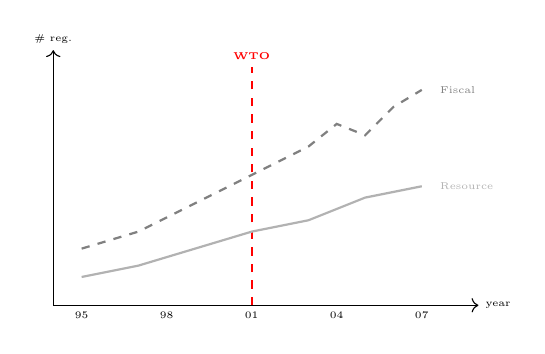
\begin{tikzpicture}[scale=0.72, transform shape]
\begin{scope}
    % Axes
    \draw[->] (0,0) -- (7.5,0) node[right] {\tiny year};
    \draw[->] (0,0) -- (0,4.5) node[above] {\tiny \# reg.};
    
    \foreach \x/\l in {0.5/95, 2/98, 3.5/01, 5/04, 6.5/07} {
        \node[below, font=\tiny] at (\x, 0) {\l};
    }
    
    % Vertical WTO line
    \draw[dashed, red, thick] (3.5,0) -- (3.5,4.2) node[above, font=\tiny\bfseries] {WTO};
    
    % Fiscal regulations - no break
    \draw[dashed, gray, thick] (0.5,1.0) -- (1.5,1.3) -- (2.5,1.8) -- (3.5,2.3) -- (4.5,2.8) -- (5,3.2) -- (5.5,3.0) -- (6,3.5) -- (6.5,3.8);
    \node[right, font=\tiny, gray] at (6.7,3.8) {Fiscal};
    
    % Resource regulations - no break
    \draw[thick, gray!60] (0.5,0.5) -- (1.5,0.7) -- (2.5,1.0) -- (3.5,1.3) -- (4.5,1.5) -- (5,1.7) -- (5.5,1.9) -- (6,2.0) -- (6.5,2.1);
    \node[right, font=\tiny, gray!60] at (6.7,2.1) {Resource};
\end{scope}
\end{tikzpicture}

\medskip
\footnotesize
Fiscal and resource regulations show \hlight{no structural break} around 2001 $\rightarrow$ rules out mechanical data-coverage explanation

\bigskip
\normalsize
\textbf{Summary (2002--07):}\\
748 new regulations; 179/340 prefectures; mean score = 1; driven by \textit{work} and \textit{social insurance} topics
\end{column}
\end{columns}
\end{frame}

% =============================================================================
\section{Trade Shock: China's WTO Accession}
% =============================================================================

\begin{frame}{Constructing the Trade Shock: Prefecture-Level Tariff Changes}
\textbf{Key variable:} Change in tariffs on Chinese exports imposed by importing countries

\bigskip
\textbf{Industry-level tariff:} Weighted average of destination-country applied tariffs (World Bank TRAINS), weights = 1995 export shares:
$$\tau_{jt}^{X} = \sum_{n} \frac{X_{j,1995}^{cn}}{\sum_{n'} X_{j,1995}^{cn'}} \cdot \tau_{jt}^{cn}$$

\bigskip
\textbf{Prefecture-level tariff change} (Kovak, 2013 style Bartik measure):
$$\Delta \text{tariffs on exports}_{it} = \sum_{j} \beta_{ij}\left[\ln(1+\tau_{jt'}^X) - \ln(1+\tau_{jt}^X)\right]$$
\vspace{-6pt}
$$\text{where } \beta_{ij} = \frac{\lambda_{ij} / \theta_{ij}}{\sum_{j'}\lambda_{ij'}/\theta_{ij'}}$$

\begin{itemize}
    \item $\lambda_{ij} = L_{ij}/L_i$: employment share of industry $j$ in prefecture $i$
    \item $1-\theta_{ij}$: cost share of labor in industry $j$ (from 2000 Industrial Enterprises Survey)
    \item Weights $\beta_{ij}$ adjust for labor intensity, following the specific-factors logic of Kovak (2013)
\end{itemize}
\end{frame}

% --- Additional Export Shocks ---
\begin{frame}{Additional Export Demand Shocks}
\textbf{Two other WTO-induced positive demand shocks:}

\bigskip
\begin{columns}[T]
\begin{column}{0.48\textwidth}
\hlight{1. PNTR Shock} (Pierce \& Schott, 2016; Handley \& Lim\~{a}o, 2017)
\begin{itemize}\setlength{\itemsep}{2pt}
    \item Pre-WTO: U.S.\ applied MFN tariffs but status reviewed annually $\rightarrow$ \rmark{policy uncertainty}
    \item WTO made MFN status permanent
    \item Measure:
\end{itemize}
\vspace{-4pt}
$$\text{PNTR}_{it} = \sum_j \beta_{ij}(\text{Col2}_j - \text{MFN}_j) \times \frac{\text{exp}_{i}^{US}}{\text{exp}_{i}^{W}}$$
\end{column}
\begin{column}{0.48\textwidth}
\hlight{2. MFA Quota Removal} (Khandelwal et al., 2013)
\begin{itemize}\setlength{\itemsep}{2pt}
    \item Textile/clothing exports to US, EU, Canada under quota until Jan.\ 2005
    \item Removal $\rightarrow$ boosted Chinese exports in these industries
    \item Measure:
\end{itemize}
\vspace{-4pt}
$$\text{MFA}_{it} = \sum_p \frac{\text{exp}_{p,i,2000}}{\sum_{p'}\text{exp}_{p',i,2000}} \cdot \mathbf{1}(\text{MFA}_p)$$
\end{column}
\end{columns}

\bigskip
\textbf{Why focus on \underline{export} tariffs?}
\begin{itemize}
    \item Decline was \textit{direct and salient} from officials' perspective
    \item China's comparative advantage in labor-intensive goods $\rightarrow$ export expansion triggers labor demand $\rightarrow$ migration regulation change
    \item Import competition mostly on high-end goods (autos, agriculture)
    \item Empirically: controls for $\Delta$ tariffs on imports and intermediate inputs included
\end{itemize}
\end{frame}

% =============================================================================
\section{Identification Strategy}
% =============================================================================

\begin{frame}{Identification Strategy: Long-Difference DiD}
\textbf{Econometric specification} (long-difference, 2001--2007):
\begin{equation*}
\boxed{\Delta\asinh(\text{regulation score})_{it} = \alpha_0 + \alpha_1 \underbrace{\Delta\text{tariffs on exports}_{it}}_{\text{Bartik measure}} + X_{it}\Gamma + \epsilon_{it}}
\end{equation*}

\medskip
\begin{itemize}
    \item $\asinh(\cdot)$: inverse hyperbolic sine transformation (handles zeros/negatives; score distribution very skewed)
    \item $X_{it}$: changes in tariffs on imports/inputs, initial regulation score, PNTR shock, MFA shock, lagged GDP/wage growth
    \item Standard errors: clustered at province level (+ bootstrap, AKM corrections)
\end{itemize}

\bigskip
\textbf{Key identification assumption:}\\[4pt]
Conditional on $X_{it}$, no unobservables correlated with $\Delta\text{tariffs on exports}_{it}$ that \textit{directly} affect regulation changes.

\bigskip
\textbf{Why is this credible?}
\begin{itemize}
    \item Post-WTO tariff cuts determined by WTO rules and importing countries' schedules $\rightarrow$ \hlight{exogenous to Chinese prefecture conditions}
    \item Cross-industry variation: tariff cuts $\neq$ predetermined by pre-WTO export growth or tariff trends
    \item Cross-prefecture variation: post-WTO tariff changes $\not\Rightarrow$ pre-WTO GDP/wage growth differences
\end{itemize}
\end{frame}

% --- Pre-Trends ---
\begin{frame}{Identification: Pre-Trend Tests}
\begin{columns}[T]
\begin{column}{0.48\textwidth}
\textbf{Industry-Level Exogeneity}

\begin{tikzpicture}[scale=0.7, transform shape]
    % Panel (a)
    \draw[->] (0,0) -- (6,0) node[right, font=\tiny] {$\Delta\ln$ exports, 95--01};
    \draw[->] (0,-1.5) -- (0,3) node[above, font=\tiny] {$\Delta$ tariff, 01--07};
    
    % Scatter dots (stylized)
    \foreach \x/\y in {0.8/0.5, 1.2/-0.3, 1.8/0.3, 2.3/0.0, 2.8/-0.2, 3.2/0.4, 3.8/-0.5, 4.2/0.1, 4.8/-0.8, 1.0/1.0, 3.5/-1.0, 2.0/0.7} {
        \fill[blue!60] (\x, \y) circle (2pt);
    }
    
    % Flat fitted line
    \draw[thick, red, dashed] (0.5,0.05) -- (5.2,0.15);
    \node[font=\scriptsize, red] at (4.5, 0.8) {Slope = 0.03};
    \node[font=\scriptsize, red] at (4.5, 0.3) {(s.e.\ = 0.3)};
\end{tikzpicture}

\medskip
\footnotesize
Industries with bigger pre-WTO export growth did \hlight{not} get bigger post-WTO tariff cuts

\bigskip
\normalsize
\textbf{Industry-Level:}
\begin{itemize}\footnotesize
    \item Post-WTO tariff $\perp$ pre-WTO export growth
    \item Post-WTO tariff $\perp$ pre-WTO tariff decline
\end{itemize}
\end{column}
\begin{column}{0.48\textwidth}
\textbf{Prefecture-Level Pre-Trends}

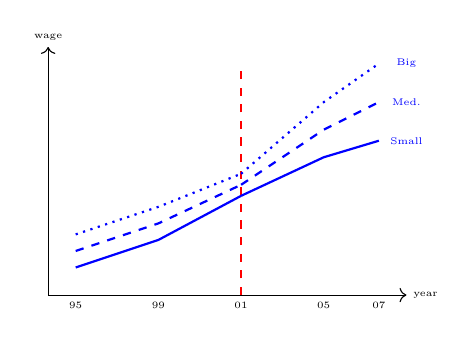
\begin{tikzpicture}[scale=0.7, transform shape]
    % Axes
    \draw[->] (0,0) -- (6.5,0) node[right, font=\tiny] {year};
    \draw[->] (0,0) -- (0,4.5) node[above, font=\tiny] {wage};
    
    \foreach \x/\l in {0.5/95, 2/99, 3.5/01, 5/05, 6/07} {
        \node[below, font=\tiny] at (\x, 0) {\l};
    }
    
    \draw[dashed, red, thick] (3.5,0) -- (3.5,4.2);
    
    % Three parallel lines pre-WTO
    \draw[thick, blue] (0.5,0.5) -- (2,1.0) -- (3.5,1.8);
    \draw[thick, blue, dashed] (0.5,0.8) -- (2,1.3) -- (3.5,2.0);
    \draw[thick, blue, dotted] (0.5,1.1) -- (2,1.6) -- (3.5,2.2);
    
    % Diverge post-WTO
    \draw[thick, blue] (3.5,1.8) -- (5,2.5) -- (6,2.8);
    \draw[thick, blue, dashed] (3.5,2.0) -- (5,3.0) -- (6,3.5);
    \draw[thick, blue, dotted] (3.5,2.2) -- (5,3.5) -- (6,4.2);
    
    \node[font=\tiny, blue] at (6.5, 2.8) {Small};
    \node[font=\tiny, blue] at (6.5, 3.5) {Med.};
    \node[font=\tiny, blue] at (6.5, 4.2) {Big};
\end{tikzpicture}

\medskip
\footnotesize
Wages parallel pre-WTO across small/medium/big tariff-decline groups. Divergence only \textit{after} 2001.

\bigskip
\normalsize
\textbf{Prefecture-Level:}
\begin{itemize}\footnotesize
    \item Wage trends: parallel pre-WTO
    \item GDP trends: slight divergence (controlled in regressions)
\end{itemize}
\end{column}
\end{columns}
\end{frame}

% =============================================================================
\section{Main Results}
% =============================================================================

\begin{frame}{Main Result: Trade Liberalization $\rightarrow$ Pro-Migrant Regulations}
\textbf{Figure 5: Scatter plot --- $\Delta$ Tariffs vs.\ $\Delta$ Regulation Score, 2001--2007}

\begin{columns}[T]
\begin{column}{0.45\textwidth}
\begin{tikzpicture}[scale=0.75, transform shape]
    \draw[->] (-0.3,0) -- (6.5,0) node[right, font=\tiny] {$\Delta$ tariffs on exports};
    \draw[->] (0,-0.5) -- (0,5.5) node[above, font=\tiny] {$\Delta\asinh$(reg.\ score)};
    
    \node[below, font=\tiny] at (0.5,0) {$-0.6$};
    \node[below, font=\tiny] at (3,0) {$0$};
    \node[below, font=\tiny] at (5.5,0) {$0.4$};
    
    % Many scatter dots
    \foreach \x/\y in {
        0.8/4.5, 1.0/3.8, 1.2/4.0, 1.5/3.2, 1.3/2.8,
        1.8/3.5, 2.0/2.5, 2.2/2.0, 2.5/1.8, 2.3/2.2,
        2.7/1.5, 2.8/1.8, 3.0/1.2, 3.2/1.0, 3.0/0.8,
        3.5/0.5, 3.3/0.7, 3.8/0.3, 4.0/0.5, 4.2/0.8,
        4.5/0.3, 4.8/0.2, 3.5/1.5, 2.0/3.0, 1.5/2.5} {
        \fill[blue!50] (\x, \y) circle (2pt);
    }
    
    % Fitted lines
    \draw[thick, red, dashed] (0.5,4.8) -- (5.5,0.0);
    \node[font=\scriptsize, red] at (1.0,5.2) {Slope $\approx -1.84$};
    
    % Labels for cities
    \node[font=\tiny, above] at (0.8,4.5) {Shanghai};
    \node[font=\tiny, right] at (1.2,4.0) {Guangzhou};
    \node[font=\tiny, above] at (1.5,3.2) {Beijing};
\end{tikzpicture}
\end{column}
\begin{column}{0.52\textwidth}
\textbf{Key finding:}\\[4pt]
\gmark{Negative and significant relationship}: prefectures with larger tariff declines $\rightarrow$ larger regulation score increases

\bigskip
\textbf{Magnitudes (Table 1, Col.\ 1):}
\begin{itemize}
    \item $\hat{\alpha}_1 = -1.04^{***}$ (s.e.\ = 0.30)
    \item 1 p.p.\ larger tariff decline $\rightarrow$ 1.04 larger $\Delta\asinh$(score) $\approx$ 1 s.d.
\end{itemize}

\bigskip
\textbf{Economic magnitude:}
\begin{itemize}
    \item Big-decline prefectures: avg.\ $-0.36$ p.p.\ tariff cut
    \item Small-decline: avg.\ $+0.04$ p.p.
    \item Difference: $0.40$ p.p.\ $\rightarrow$ \rmark{0.40 s.d.}\ larger regulation score increase
\end{itemize}

\bigskip
\textbf{Pre-WTO placebo:}\\
Slopes $= -0.01$ to $0.04$, \textit{insignificant}
\end{column}
\end{columns}
\end{frame}

% --- Regression Table ---
\begin{frame}{Table 1: Main Regression Results (Selected Columns)}
\begin{table}[h]
\centering\footnotesize
\setlength{\tabcolsep}{3pt}
\begin{tabular}{@{}l*{5}{c}@{}}
\toprule
& (1) & (2) & (5) & (6) & (7) \\
\midrule
\multicolumn{6}{@{}l}{\textit{Panel A. Dep.\ var.: $\Delta\asinh$(regulation score), manual coding}} \\[3pt]
$\Delta$ tariffs on exports, 01--07 & $-1.04^{***}$ & $-0.91^{***}$ & $-1.60^{***}$ & $-1.38^{***}$ & $-1.02^{*}$ \\
& (0.30) & (0.26) & (0.50) & (0.49) & (0.53) \\[3pt]
PNTR shock & & $4.67^{***}$ & & $2.89^{**}$ & 1.03 \\
& & (1.44) & & (1.27) & (1.21) \\[3pt]
MFA shock & & $5.43^{***}$ & & $4.20^{**}$ & $4.86^{**}$ \\
& & (1.94) & & (1.91) & (2.25) \\[3pt]
$\Delta$ log wage, 95--01 & & & & & 0.69 \\
$\Delta$ log GDP p.c., 95--01 & & & & & $0.65^{***}$ \\[3pt]
\midrule
Prefectures & 333 & 333 & 248 & 248 & 235 \\
$R^2$ & 0.09 & 0.14 & 0.08 & 0.11 & 0.15 \\
Bootstrap $p$ & .006 & .005 & .006 & .014 & .078 \\
AKM(0) $p$ & .024 & .020 & .036 & .055 & .051 \\
\midrule
\multicolumn{6}{@{}l}{\textit{Panel B. Random Forest coding: $\hat{\alpha}_1$ ranges from $-1.39^{***}$ to $-0.89^{*}$}} \\
\bottomrule
\end{tabular}
\end{table}

\medskip
\footnotesize
All columns control for $\Delta$ tariffs on imports, $\Delta$ tariffs on inputs, initial score. SE clustered at province.\\
Cols 5--7 restrict to 248 prefectures in Prefecture Statistics Yearbook (more urban).
\end{frame}

% =============================================================================
\section{Heterogeneous Effects}
% =============================================================================

\begin{frame}{Heterogeneous Effects: Who Responds More?}
\textbf{Specification:}
$$\Delta\asinh(\text{reg.\ score})_{it} = \beta_0 + \beta_1 \Delta T_{it} + \beta_2 I_{it} + \beta_3 \underbrace{I_{it} \times \Delta T_{it}}_{\text{interaction}} + X_{it}\Gamma + \epsilon_{it}$$

\medskip
\begin{columns}[T]
\begin{column}{0.48\textwidth}
\begin{table}[h]
\centering\scriptsize
\setlength{\tabcolsep}{2pt}
\begin{tabular}{@{}lcccc@{}}
\toprule
Baseline & Migrant & Private & GDP & Wage \\
characteristic $I$: & intensity & firm share & p.c. & \\
\midrule
$\hat{\beta}_1$ ($\Delta T$) & 4.65 & 1.21 & $10.98^*$ & 29.53 \\
& (3.65) & (0.72) & (5.97) & (18.72) \\[3pt]
$\hat{\beta}_3$ ($\Delta T \times I$) & $-17.31$ & $-5.47^{***}$ & $-1.29^*$ & $-3.33$ \\
& (10.93) & (1.09) & (0.68) & (2.07) \\[3pt]
\midrule
Effect at mean $I$: & $-1.24$ & $-1.80$ & $-0.55$ & $-0.81$ \\
$N$ & 248 & 248 & 248 & 248 \\
\bottomrule
\end{tabular}
\end{table}
\end{column}
\begin{column}{0.48\textwidth}
\textbf{Interpretation:}
\begin{itemize}\setlength{\itemsep}{4pt}
    \item[\gmark{$\checkmark$}] \textbf{Migrant-intensive} prefectures respond more strongly
    \item[\gmark{$\checkmark$}] Higher \textbf{private-firm share} $\rightarrow$ stronger response (SOEs hire fewer migrants)
    \item[\gmark{$\checkmark$}] \textbf{Richer} prefectures respond more (higher income $\approx$ higher migrant demand)
\end{itemize}

\bigskip
\rmark{Reinforces the mechanism:} prefectures that \textit{needed} migrants most were the ones that responded to tariff cuts by relaxing Hukou restrictions
\end{column}
\end{columns}
\end{frame}

% =============================================================================
\section{De Facto Effects: Migrant Well-Being}
% =============================================================================

\begin{frame}{Do Regulations Matter? Evidence on Migrant Well-Being (2005)}
\textbf{Question:} Are these \textit{de jure} regulation changes also \textit{de facto} effective?\\[3pt]
\textbf{Data:} 2005 1\% Population Survey (cross-section)

\begin{table}[h]
\centering\footnotesize
\setlength{\tabcolsep}{3pt}
\begin{tabular}{@{}lcccccc@{}}
\toprule
Dep.\ var.\ (migrants): & Unemp.\ & Pension & Medical & Contract & Monthly & School \\
& Ins.\ rate & rate & Ins.\ rate & (months) & Income & Enroll. \\
\midrule
$\asinh$(reg.\ score)$_{2005}$ & $0.01^*$ & $0.02^{**}$ & $0.02^{**}$ & 0.09 & $29.27^{**}$ & 0.00 \\
& (0.01) & (0.01) & (0.01) & (0.10) & (13.98) & (0.00) \\[3pt]
Local well-being control & \gmark{Yes} & \gmark{Yes} & \gmark{Yes} & \gmark{Yes} & \gmark{Yes} & \gmark{Yes} \\
\midrule
Mean (migrants) & 0.21 & 0.34 & 0.36 & 4.57 & 923 & 0.94 \\
Mean (locals) & 0.37 & 0.60 & 0.59 & 5.05 & 981 & 0.95 \\
\bottomrule
\end{tabular}
\end{table}

\medskip
\textbf{Key takeaways:}
\begin{itemize}
    \item 1 s.d.\ $\uparrow$ regulation score: unemployment insurance gap closes by \hlight{6.25\%}; income rises \hlight{29 yuan/month} ($\approx$ 50\% of migrant-local wage gap)
    \item Effects significant for \textit{workplace} outcomes (insurance, wages); \textit{not} for school enrollment
    \item Local well-being \textit{not} significantly affected (Cols 1--3, 5 in Panel B) $\rightarrow$ regulation captures \textit{migrant-specific} improvement
\end{itemize}
\end{frame}

% =============================================================================
\section{Trade, Regulation, and Migrant Flows}
% =============================================================================

\begin{frame}{From Regulations to Migrant Flows}
\textbf{Reduced-form:} $\Delta Y_{it} = \gamma_0 + \gamma_1 \Delta\text{tariffs on exports}_{it} + X_{it}\Gamma + \xi_{it}$

\textbf{Association:} $\Delta Y_{it} = \pi_0 + \pi_1 \Delta\asinh(\text{reg.\ score})_{it} + X_{it}\Phi + \zeta_{it}$

\begin{table}[h]
\centering\footnotesize
\setlength{\tabcolsep}{3pt}
\begin{tabular}{@{}l*{6}{c}@{}}
\toprule
& \multicolumn{3}{c}{$\Delta$ Migrant share of pop.} & \multicolumn{3}{c}{$\Delta\ln$ \# migrants (short dist.)} \\
\cmidrule(lr){2-4}\cmidrule(lr){5-7}
& (1) & (2) & (3) & (4) & (5) & (6) \\
\midrule
$\Delta$ tariffs on exports & $-7.11^{**}$ & & $-6.23^*$ & $-1.34^{***}$ & & $-1.18^{***}$ \\
& (3.39) & & (3.22) & (0.31) & & (0.27) \\[3pt]
$\Delta\asinh$(reg.\ score) & & $1.03^{***}$ & $0.87^{***}$ & & $0.18^{***}$ & $0.20^{***}$ \\
& & (0.29) & (0.22) & & (0.04) & (0.04) \\
\bottomrule
\end{tabular}
\end{table}

\medskip
\textbf{Results by Migration Distance:}
\begin{itemize}
    \item \textbf{Short-distance:} Both trade and regulations significant
    \item \textbf{Medium-distance:} Trade effect significant; regulation effect marginally significant
    \item \textbf{Long-distance:} Trade effect \textit{insignificant}; regulation effect \textit{significant}
\end{itemize}

\rmark{$\Rightarrow$} For long-distance migration, \hlight{regulatory amenities may matter more than prices}

\medskip
\footnotesize
\textit{Caveat:} $\pi_1$ is \underline{not} causal (simultaneous determination, reverse causality). See Appendix C.11 for IV attempts using natural pop.\ growth rate.
\end{frame}

% =============================================================================
\section{Robustness and Extensions}
% =============================================================================

\begin{frame}{Robustness Checks: A Comprehensive Battery}

\begin{columns}[T]
\begin{column}{0.48\textwidth}
\textbf{Measurement Robustness:}
\begin{itemize}\setlength{\itemsep}{3pt}
    \item[\gmark{$\checkmark$}] NLP codings (RF, MLP, CNN, average): Table C1 --- nearly identical results
    \item[\gmark{$\checkmark$}] 3-point scale ($\{-1,0,1\}$) instead of 5-point: Table C4
    \item[\gmark{$\checkmark$}] Score levels instead of $\asinh$: Table C3
    \item[\gmark{$\checkmark$}] Topic decomposition: work \& public goods most affected (Table C4, Cols 4--8)
\end{itemize}

\bigskip
\textbf{Specification Robustness:}
\begin{itemize}\setlength{\itemsep}{3pt}
    \item[\gmark{$\checkmark$}] Stacked long-difference (1995--01 + 2001--07 panel): Table C2
    \item[\gmark{$\checkmark$}] Alternative Bartik weights ($\lambda_{ij}$ only): Table C5, Col 2
    \item[\gmark{$\checkmark$}] Autor et al.\ (2013) style IPW measures: Table C5, Cols 3--7
    \item[\gmark{$\checkmark$}] GDP-based and gravity-based IV for export growth: Table C5, Cols 6--7
\end{itemize}
\end{column}
\begin{column}{0.48\textwidth}
\textbf{Identification Robustness:}
\begin{itemize}\setlength{\itemsep}{3pt}
    \item[\gmark{$\checkmark$}] Adding industry employment shares one-at-a-time: Figure C4 --- stable around $-1.60$
    \item[\gmark{$\checkmark$}] Bootstrap SEs and AKM(0), AKM(1) corrections: similar $p$-values
    \item[\gmark{$\checkmark$}] Pre-WTO placebo: slopes $\approx 0$, insignificant (Figure C2)
\end{itemize}

\bigskip
\textbf{Strategic Interaction:}
\begin{itemize}\setlength{\itemsep}{3pt}
    \item[\gmark{$\checkmark$}] Prefectures respond to tariff \& regulation changes in \textit{same-province} peers (Table C6)
    \item[\gmark{$\checkmark$}] Strongest competition among prefectures with similar \textit{GDP levels} (Table C7)
    \item Consistent with Tiebout-style fiscal competition within income tiers
\end{itemize}
\end{column}
\end{columns}
\end{frame}

% =============================================================================
\section{Discussion and Conclusion}
% =============================================================================

\begin{frame}{The Economic Logic: Putting It All Together}
\begin{center}
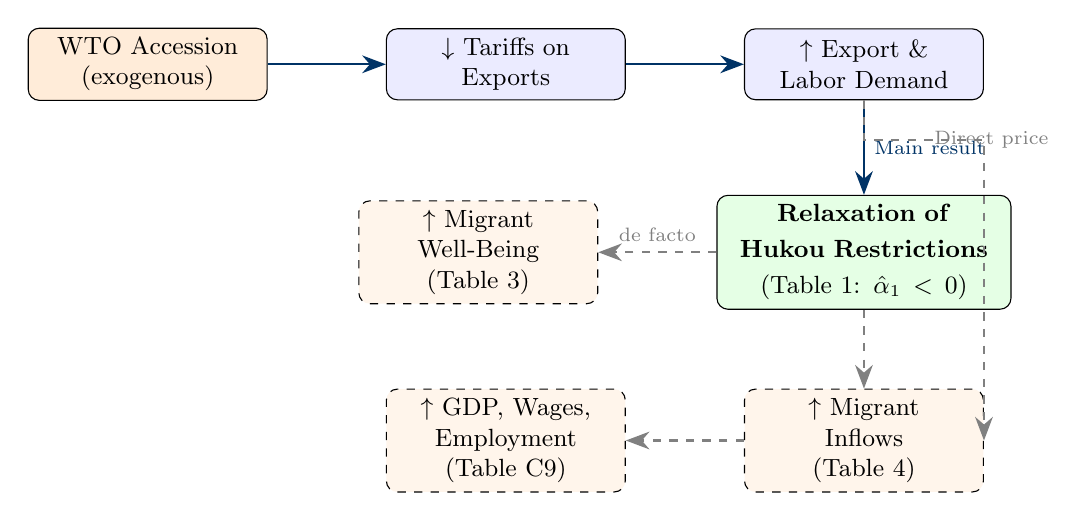
\begin{tikzpicture}[
    node distance=0.9cm and 1.2cm,
    every node/.style={font=\small},
    box/.style={draw, rounded corners, fill=blue!8, text width=2.8cm, align=center, minimum height=0.9cm},
    widebox/.style={draw, rounded corners, fill=green!10, text width=3.5cm, align=center, minimum height=0.9cm},
    dashedbox/.style={draw, dashed, rounded corners, fill=orange!8, text width=2.8cm, align=center, minimum height=0.9cm},
    arrow/.style={-{Stealth[length=3mm]}, thick, darkblue},
    darrow/.style={-{Stealth[length=3mm]}, thick, dashed, gray}
    ]
    
    \node[box, fill=orange!15] (wto) {WTO Accession\\(exogenous)};
    \node[box, right=1.5cm of wto] (tariff) {$\downarrow$ Tariffs on\\Exports};
    \node[box, right=1.5cm of tariff] (demand) {$\uparrow$ Export \&\\Labor Demand};
    
    \node[widebox, below=1.2cm of demand] (reg) {\textbf{Relaxation of}\\[2pt]\textbf{Hukou Restrictions}\\[2pt](Table 1: $\hat{\alpha}_1 < 0$)};
    
    \node[dashedbox, left=1.5cm of reg] (wellbeing) {$\uparrow$ Migrant\\Well-Being\\(Table 3)};
    \node[dashedbox, below=1.0cm of reg] (flows) {$\uparrow$ Migrant\\Inflows\\(Table 4)};
    \node[dashedbox, left=1.5cm of flows] (growth) {$\uparrow$ GDP, Wages,\\Employment\\(Table C9)};
    
    \draw[arrow] (wto) -- (tariff);
    \draw[arrow] (tariff) -- (demand);
    \draw[arrow] (demand) -- (reg) node[midway, right, font=\scriptsize] {Main result};
    \draw[darrow] (reg) -- (wellbeing) node[midway, above, font=\scriptsize] {de facto};
    \draw[darrow] (reg) -- (flows);
    \draw[darrow] (demand.south) -- ++(0,-0.5) -| (flows.east) node[near start, right, font=\scriptsize] {Direct price};
    \draw[darrow] (flows) -- (growth);
\end{tikzpicture}
\end{center}

\medskip
\textbf{Central insight:} Trade liberalization affects the economy not only through \textit{prices} but also through \textit{institutional change}. Labor market frictions are \hlight{endogenous} to trade policy.
\end{frame}

% --- Conclusion ---
\begin{frame}{Conclusion and Open Questions}
\textbf{Summary of Findings:}
\begin{enumerate}\setlength{\itemsep}{3pt}
    \item WTO-induced tariff reductions on Chinese exports caused local governments to enact \hlight{pro-migrant regulations} (0.40 s.d.\ difference between high- and low-exposure prefectures)
    \item Effect is stronger for migrant-intensive, private-sector-dominated, richer prefectures
    \item Regulations associated with improved migrant well-being (insurance, wages) and increased migrant inflows
    \item Prefectures \textit{compete} for migrants with similar-income peers
\end{enumerate}

\bigskip
\textbf{Open Questions and Limitations:}
\begin{itemize}\setlength{\itemsep}{3pt}
    \item Cannot cleanly separate direct price channel from indirect regulation channel on migrant flows
    \item De jure $\neq$ de facto: only cross-sectional evidence on enforcement (2005)
    \item Welfare implications: Is inter-prefecture competition efficiency-enhancing or a race to the bottom?
    \item Broader institutional effects of WTO: rule of law, transparency, property rights?
    \item External validity: Does the mechanism extend to other countries with internal migration barriers (Vietnam, Russia)?
\end{itemize}
\end{frame}

% --- Thank You ---
\begin{frame}[plain]
\begin{center}
\vspace{2cm}
{\LARGE\bfseries Thank You}

\bigskip
{\large Questions \& Discussion}

\bigskip\bigskip
\footnotesize
Paper: Tian, Y.\ (2024). ``International Trade Liberalization and Domestic Institutional Reform.''\\
\textit{The Review of Economics and Statistics}, 106(3): 794--813.\\[4pt]
DOI: \texttt{10.1162/rest\_a\_01175}
\end{center}
\end{frame}

\end{document}
